% \chapter{Introduction}\label{sec:1}
\section{The Ik language}\label{sec:1.1}  
Ik is the native language of the Ik people who live on a narrow swath of land in the northeastern corner of Uganda, East Africa. The people call their language \textit{Icétôd}, which means ‘Ik-speech’ or ‘Ik-talk’ and is pronounced \textit{ee-CHAY-TOad} or in phonetic symbols, [\={i}tʃétôd̻]. Ik belongs to a small cluster of languages called ‘Kuliak’, which also includes Nyang’ía of Lobalangit and Soo/Tepeth of Mounts Moroto, Napak, and Kadam – all in Uganda’s magnificent Karamoja Region. 

At the outset, let me state definitively that Ik is \textit{not }a \isi{dialect} of Karimojong, nor is it even Nilotic or ‘Hamitic’. And it is certainly not Bantu (as some have asked me). Scholars disagree as to whether it is related to Karimojong at all, but if it is, it would be a distant relationship within the great Nilo-Saharan language family, much as English is related to Russian or Hindi within Indo-European.

One reason people assume Ik is a \isi{dialect} of Karimojong is that the Ik have long been surrounded and dominated by the pastoralist Dodoth, Toposa, Turkana, and Jie. These groups, as well as the Karimojong proper, all speak mutually intelligible forms of a speech variety called ‘Ateker’, ‘Teso-Turkana’, or ‘Tunga’. Another reason Ik seems similar to Karimojong is that it has borrowed many hundreds of words from Teso-Turkana speech varieties over the centuries. In addition to lexical borrowing, the close contact between the Ik and Teso-Turkana peoples has caused Ik grammar to become more like Teso-Turkana in various ways.

But despite the many superficial similarities one may see between Ik and Teso-Turkana, their grammatical systems are actually quite different. For instance, while their vowel inventories are similar, Ik has many more consonants than Teso-Turkana, including the ejectives /ƙ/ and /tsʼ/, which are found in no other Ugandan language. Ik also has an elaborate case system with eight cases all marked with suffixes, whereas Teso-Turkana languages mark only four cases, some using only tone to do so. And although both Ik and Teso-Turkana order their words as Verb-Subject-Object in main clauses, in subordinate clauses, Ik changes the order to Subject-Verb-Object. These are but a few examples among others that show the significant differences between Ik and Teso-Turkana.

 
\section{The dictionary}\label{sec:1.2} 

This book contains a bilingual Ik-English dictionary and an English-Ik reversal index. The dictionary section lists all the Ik words I have recorded up to now and offers English definitions for them. Including proper names, there are approximately 8,700 entries in the dictionary. While I have done all I could to collect as many words as possible within the limits of time and resources, no doubt many hundreds of other words still lurk out there in the recesses of Ikian minds. It will not be until more texts are written in Ik that these missing words might be gently coaxed out onto the page and into more books like the present one. 

Although the presumed purpose of a dictionary is to propound the current meanings of the words of a language, I fear that purpose is only partly achieved in this volume. The true meanings of words are lived meanings, intended by living beings in a living world. To capture them on a page is to encase them in black rock and white ice. A native speaker of Ik may recognize in my English definitions familiar traces of true meaning but never all of it. As a foreign, non-native speaker of the language, my grasp of the living meanings of Ik words is severely limited. For the only way to learn living linguistic meanings is to experience life linguistically, \textit{through} a language, through its words and phrases and tropes. Still, I have been fortunate enough to have had a few real-life experiences in Ik, for instance, when I learned the living meaning of the verb \textit{ɨsɛɛs }‘to miss’ by actually missing a bushpig boar as I tried to spear it when it charged toward me out of a thicket. The young Ik hunters never let me forget that miss, and as they retold the story with glee, they always used that particular verb. So when I hear it, I not only know what it means in terms of ‘missing’, but I also \textit{feel} the living overtones that include shame, regret, loss of opportunity, diminution of manhood, and so on. \textit{That} is how one learns the meanings of words. 

Due to the exceptional nature of such experiences, most of the Ik words in this volume I have had to define extrinsically, from the outside. Unfortunately, as a foreign lexicographer, \textit{I do not inhabit the words}. All I could really do was try to understand the words as best I could and render them in perspicacious English, marking out a felicitous meeting place between two very different modes of linguistic being-in-the-world. To the degree that I succeeded in this endeavor, this is what I hope to be a worthwhile first full-scale Ik-English lexicon.

The English definitions the reader will find are of various types. Some Ik words lend themselves easily to one-word, entirely accurate glosses, for example, \textit{gʉɓ\'{ɛ}rá- }as ‘leopard’. Others require a short phrase in English, for instance, \textit{ƙóré- }as the ‘back of the knee’. Still others, the ones that are conceptually more distant from English, call for longer descriptions, as when \textit{makúlí- }is defined as a ‘round grass beehive cover that goes over the end of a hollow beehive’.

As well as being a record of modern Ik to be used for modern purposes, this dictionary also provides much data for historical research. Because the Ik have left little in the way of archaeology over the ages, and because oral histories tend to be vague, inconsistent, and undated, language is one of the few lenses through which to investigate prehistory. Already the Ik lexicon gives some tantalizing hints as to the ancient northern East African origins of the Ik, for example in the link between words like \textit{sɔk\'{ɔ}- }‘hoof’ and Arabic \textit{saaq }‘foot’ and Gumuz \textit{tʃagw }‘foot’, or between \textit{ƙ{\Í}dz- }‘bite’ and Maltese Arabic \textit{gidem }‘bite’ and Uduk \textit{kʼ\={u}c\={u}r }‘suck’. Every Ik word is a cultural relic, a linguistic artifact sticking out of the red clays of time and memory. Each one has been molded by a million mouthings, much as grains of sand are ground down by wind and water. Each has its own history, an origin and a tortuous path of descent to its present form, the same path, we can assume, that its many speakers have taken. This is where the fields of etymology and historical linguistics (or ‘paleolinguistics’) can provide some evidence on which to build a grounded sense of identity and cultural history.

A deeply rooted sense of history and identity is important because it could help give the Ik a more sure footing as they transition into a nationally-minded Ugandan society and a globally-minded international society. If I imagine the future fate of the Ik language, I can see two possible developmental paths it could take. The first is that it could be lost by being totally assimilated by Karimojong, much like Nyang’ía already has and Soo/Tepeth is in danger of doing, or by succumbing to the dazzling promise of upward mobility that English seems to offer. If either of these forms of language death should take place, at least this book would remain as a monument to a once noble language-mediated world-view.

   

\begin{figure}
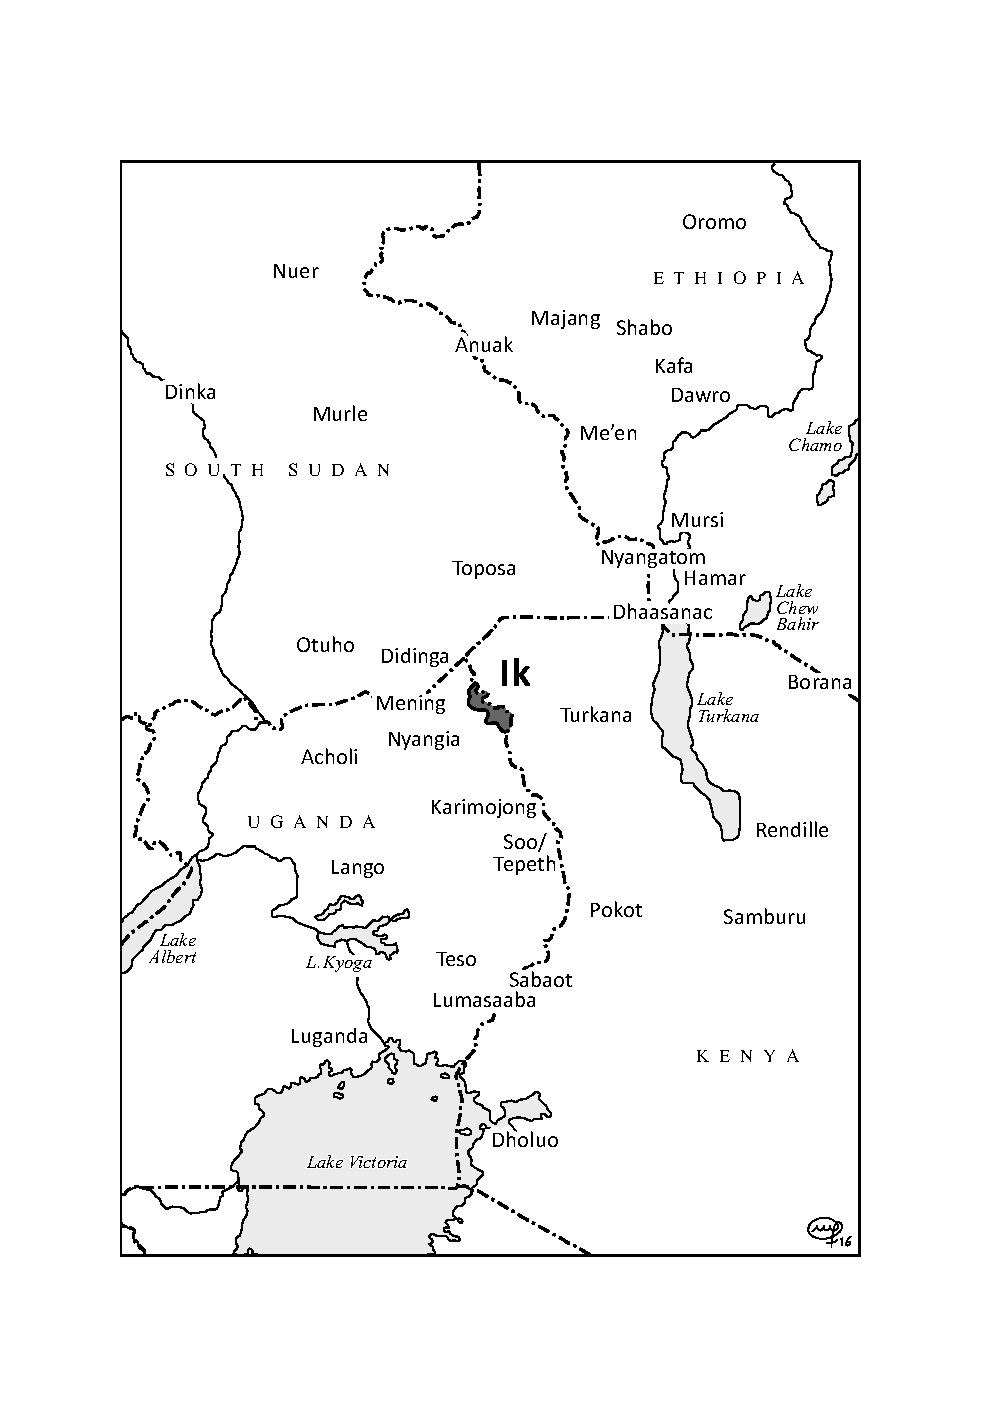
\includegraphics[width=\textwidth]{figures/Uganda_Ik_2016_Schrock.pdf}
\caption{Ik language area in an ‘Ik-centric’ perspective \tiny{(CC-BY Monika Feinen)}}
\label{fig:1}
\end{figure}

The second path the Ik language could take into the future is the one I have often daydreamed of. It is the one that would fulfill my scholarly strivings and confirm my greatest hopes for the Ik. In this path, Ik would go on to become the language of a highly literate populace who would use it skillfully to promote their own well-being. With explicit knowledge of their grammar and lexicon, educated Ik people would harness the expressive power of their native-born tongue and make it a vehicle of music, poetry, fiction, philosophy, theology, medicine, education, policy – the full gamut of human expression. This scrappy language that has barely scraped by countless threats to its existence yet somehow managed to pull through, this language that contains the linguistic genes of so many other languages from unrelated stocks, this small language of a small people in small place, could go on to become an enduring symbol of the Ikian spirit. 

As portrayed in \figref{fig:1}, the Ik language area can be viewed imaginatively from an ‘Ik-centric’ perspective as a ‘heart’ of East Africa. There it lies, near the arterial convergence of four East African nations: Uganda, South Sudan, Ethiopia, and Kenya. Over the centuries the Ik have migrated through and throughout each of these four countries. While doing so, their language absorbed words and grammatical traits from the many languages spoken there. So, in a real sense, Ik embodies the linguistic heritage of northern East Africa. Thus, could it  be that Ik is providentially situated to blossom into a language that can serve the full range of communicative needs of a modernized Ik society, and then extend its fruited boughs over the escarpment in four directions to become a blessing to the neighboring nations? In the end, only time will tell, and yet it is toward the fulfillment of that dream that this work on Ik has been lovingly consecrated.
 
\section{Using the dictionary}\label{sec:1.3}
\subsection{Writing system}\label{sec:1.3.1}

The Ik script used in this dictionary and grammar sketch is based on what is called the Linguistic Orthography (LingO) as described in \citet{Schrock2015}. The LingO is a compromise between the simpler Popular Orthography (PopO) and a more scientific writing system. The main reason for choosing the LingO over the PopO is that the LingO encodes three very important features of the Ik sound system: voiceless vowels, \isi{vowel harmony}, and tone. Although these three features are difficult to remember and write, they are indispensable for the correct pronunciation of Ik. Therefore it was decided that for this book to be an accurate and reliable record of the language, the proper pronunciations would have to be reflected in the spellings. LingO writing can easily be converted to PopO, but the reverse is not true, since it requires greater linguistic awareness.

The alphabetical order of Ik letters is given below. Note that the vowel pairs E/Ɛ, I/Ɨ, O/Ɔ, and U/Ʉ – whose two members differ only in terms of a linguistic feature called Advanced Tongue Root [\isi{ATR}] – are alphabetized as if they were the same letter. This is done to assist non-native speakers of Ik in finding words beginning with vowels they might not be able to distinguish at first. Also note that the letter (Ʒ) is in parentheses because even though it belongs to the alphabet, no recorded Ik word begins with it. For the pronunciation of these letters, the reader is referred ahead to \sectref{sec:2.1} of the grammar sketch section.
 
\begin{itemize}
\item  Ik alphabetical order: A B Ɓ C D Ɗ Dz E/Ɛ F G H Hy I/Ɨ J Jʼ K Ƙ L M N Ɲ Ŋ O/Ɔ P R S T Ts Tsʼ U/Ʉ W X Y Z (Ʒ)
\end{itemize}
 
\subsection{Structure of entries}\label{sec:1.3.2}

The Ik-English dictionary section contains entries of the following kinds of Ik words\textsc{:} nouns, pronouns, demonstratives, quantifiers, numerals, prepositions, verbs, adverbs, ideophones, interjections, nursery words, complementizers, and connectives (or conjunctions). For a brief description of each word class, the reader is referred to \sectref{sec:3} of the grammar sketch at the back of the book. The goal of the present section is to explain to the user the structure of lexicographical entries. To do this, an example of a noun entry and a verb entry are discussed.

A typical noun entry has several components. To identify them, match the numbered components in this explanatory paragraph with the superscript number in the model entry below. 1) The lexical headword is in bold typeface. It is the citation form of the noun, that is, the form of the noun spoken in isolation. In Ik, the citation form takes the \isi{nominative case} (see \sectref{sec:7.2}). 2) The root or lexical form is in parentheses. It is hyphenated to show that it still needs a case ending, and it is the form on which to base all other case forms of this noun. This particular noun is also hyphenated in the middle to signify that it is a compound noun made of two parts (see \sectref{sec:4.3} of the grammar). 3) This is an abbreviation for ‘plural’, indicating that the next item is the plural form of the headword. 4) This is the plural form of the singular headword \textit{bàdìàm}. 5) This number (1) indicates that what follows is the first and primary sense or meaning of the headword. 6) This is an abbreviation of the grammatical category of the word, in this case \textit{n.} for ‘noun’. 7) After the primary sense, one or more other numbered senses of the word may be added. 8) After the senses, one or more notes may mention further information about the entry, for example cultural details or suggestions for synonyms or near-synonyms.

\dicobox{
\textbf{\textsuperscript{1}}\textbf{bàdìàm }\textsuperscript{2}(bàdì-àmà-)\textit{ }\textsuperscript{3}\textit{pl.}\textsc{ }\textsc{\textsuperscript{4}}badiikᵃ \textsuperscript{5}1) \textsuperscript{6}\textit{n. }sorcerer, wizard \textsuperscript{7}2) anything spooky, weird, or uncanny {\textbar} \textsuperscript{8}The concept of \textit{bàdìàm} includes nocturnal animals like bats, hyenas, and owls that have strange characteristics... tobacco is also called \textit{bàdìàm} because its strong physiological effects are not attributable to human agency.
}

A typical verb entry has similar components but also some different ones: 1) Just as with nouns, the verbal headword is shown in bold typeface. This is the citation form of the verb, which in Ik appears in the \isi{infinitive} form and \isi{nominative case} (see \sectref{sec:8.2} in the grammar). As an \isi{infinitive}, the verb is acting as a noun at this point, much like ‘to go’ or ‘going’ in English. To use an Ik \isi{infinitive} as a verb, simply remove the \isi{infinitive} suffix (either \textit{-ònì- }or \textit{-ésí-}) and use the appropriate suffixes (see \sectref{sec:8.7}). 2) Then, the form in the parentheses is the lexical form of the infinitival headword, the one that is the base for all other case-inflected forms of the verb. 3) This number (1) indicates that what follows is the first and primary sense or meaning of the headword. 4) This is an abbreviation of the grammatical category of the headword, in this case \textit{v. }for ‘verb’. 5) After the primary sense, one or more other senses of the headword may be added. 6) This short note directs the user to a synonym or near-synonym of the headword.

\dicobox{
\textbf{\textsuperscript{1}}\textbf{betsínón }\textsuperscript{2}(betsínónì-) \textit{ }\textsuperscript{3}1) \textsuperscript{4}\textit{v. }to be awkward, gauche, inept \textsuperscript{5}2) to be left-handed, sinistral {\textbar} \textsuperscript{6}See also \textit{ɨɓaŋɨɓáŋɔn}. 
}

Over a hundred Ik verb roots end in /a/, /e/, or /ɛ/, meaning that when an \isi{infinitive} suffix is added to the root, these root-final vowels are assimilated (see \sectref{sec:2.4.4}). For example, though the root for ‘miss’ is \textit{ɨsá-}, the \isi{infinitive} form is \textit{ɨsɛɛs}, which obscures the root-final vowel. Lest the dictionary user hear a form of the root \textit{ɨsá-} in speech and then fail to deduce that its \isi{infinitive} is \textit{ɨsɛɛs}, both root and \isi{infinitive} have been listed in the dictionary. The entry for \textit{ɨsá-} includes the notation (<ɨsɛɛs) which indicates that \textit{ɨsɛɛs }is the entry the user should go to for the definition. Conversely, the entry for \textit{ɨsɛɛs} ‘to miss’ includes both the lexical form of the \isi{infinitive} and the bare root, as in: \textbf{ɨsɛɛs}\textit{ }(ɨsɛɛs{\Í}-/ɨsá-). 
 
\subsection{Tips for finding words}\label{sec:1.3.3}

Finally, because a good number of Ik words have more than one form, and because many of them can be reasonably spelled in multiple ways, let me offer the user the following tips for locating polymorphous words in the dictionary:

\begin{itemize}
\item 
If you are looking up a verb beginning with /i/ or /ɨ/ and cannot find it, remove the /i/ or /ɨ/ and try again. Conversely, if you are looking up a verb and cannot find it, try adding an /i/ or /ɨ/ to see if that takes you to a word.
\item 
If you are looking up a word beginning with /w/ and cannot find it, try replacing the /w/ with /ɔ/, /o/, /ʉ/, or /u/ and vice versa.
\item
If you are looking up a word beginning with /y/ and cannot find it, try placing the /y/ with /i/ or /ɨ/ and vice versa. 
\item 
If you are looking up a noun beginning with /ɲa/ and cannot find it, try replacing it with /ɲe/ and vice versa. 
\item 
If you are looking up a noun beginning with /ɲe/ and cannot find it, try replacing it with /ɲo/ and vice versa. 
\item 
If you are looking up a word beginning with /ts/ and cannot find it, try replacing it with /tsʼ/ and vice versa. 
\item 
If you are looking up a word beginning with /dz/ and cannot find it, try replacing it with /ts/ or /tsʼ/ and vice versa. 
\item 
If you are looking up a word beginning with /d/ and cannot find it, try replacing it with /ɗ/ or /t/ and vice versa. 
\item 
If you are looking up a word beginning with /g/ and cannot find it, try replacing it with /ƙ/ or /ŋ/ and vice versa. 
\item 
If you are looking up a word containing the vowels /e, i, o, u/ and cannot find it, try replacing the vowel with /ɛ, ɨ, ɔ, ʉ/.
\end{itemize}
 
